\section{Angular analysis}
The forward-backward asymmetries of both the dimuon system, $A_{\rm
  FB}^\ell$, and of the $p\pi$ system, $A_{\rm FB}^h$, are defined as
\begin{align}
A_{\rm FB}^i(\qsq)&=\frac{\int_0^1 \frac{\deriv^2\Gamma}{\deriv\qsq\,\deriv\!\cos\theta_i} \deriv\!\cos\theta_i-
               \int^0_{-1} \frac{\deriv^2\Gamma}{\deriv\qsq\,\deriv\!\cos\theta_i} \deriv\!\cos\theta_i}{\deriv\Gamma / \deriv \qsq},
\label{eq:afbTh}
\end{align}
\noindent
where $\deriv^2\Gamma/\deriv q^2\,\deriv\!\cos\theta_i$ is the
two-dimensional differential rate and $\deriv\Gamma/\deriv q^2$ is the
rate integrated over the corresponding angles.  The observables are
determined by a fit to one-dimensional angular distributions as a
function of $\cos \theta_\ell$, the angle between the positive
(negative) muon direction and the dimuon system direction in the
\Lb(\Lbbar) rest frame, and $\cos \theta_h$, which is defined as the
angle between the proton and the \Lz baryon directions, also in the
\Lb rest frame. The differential rate as a function of $\cos
\theta_\ell$ is described by the function
\begin{align}
\frac{\deriv^2\Gamma(\Lambda_{b}\to \Lambda \,\ell^{+}\ell^{-})}{\deriv\qsq\,\deriv\!\cos\theta_\ell}=
\frac{\deriv\Gamma}{\deriv\qsq}&\left[  \frac{3}{8}\left(1+\cos^2\theta_\ell\right)(1-f_{\rm L})+A_{\rm FB}^\ell\cos\theta_\ell +
   \frac{3}{4}f_{\rm L} \sin^2\theta_\ell \right], 
\label{eq:afbLTh}
\end{align}
where $f_{\rm L}$ is the fraction of longitudinally polarised dimuons.
 The rate as a function of $\cos \theta_h$ has the form
\begin{equation}
\frac{\deriv^2\Gamma(\Lambda_{b}\to \Lambda(\to p \pi^{-})\ell^{+}\ell^{-})}
     {\deriv\qsq\,\deriv\!\cos\theta_h} 
={\BF}(\Lambda \to p\pi^{-})
 \frac{\deriv\Gamma(\Lambda_b \to \Lambda\, \ell^{+}\ell^{-})}{\deriv \qsq}\frac{1}{2}
\Big(1+2A_{\rm FB}^h\cos\theta_h\Big) \,.
\label{eq:afbBTh}
\end{equation}
\noindent
These expressions assume that \Lb baryons are produced unpolarised,
which is in agreement with the measured production polarisation at
\lhcb~\cite{LHCb-PAPER-2012-057}.

The forward-backward asymmetries are measured in data using unbinned
maximum likelihood fits.  The signal PDF consists of a theoretical
shape, given by Eqs.~\ref{eq:afbLTh} and \ref{eq:afbBTh}, multiplied
by an acceptance function.  Selection requirements on the minimum
momentum of the muons may distort the $\cos \theta_\ell$ distribution
by removing candidates with extreme values of $\cos
\theta_\ell$. Similarly, the impact parameter requirements affect
$\cos \theta_h$ as very forward hadrons tend to have smaller impact
parameter values.  The angular efficiency is parametrised using a
second-order polynomial and determined separately for downstream and
long candidates by fitting simulated events, with an independent set
of parameters obtained for each \qsq interval. These parameters are
fixed in the fits to data.  The acceptances are shown in
Fig.~\ref{fig:AngEff} as a function of $\cos\theta_h$ and
$\cos\theta_\ell$ in the $15 < \qsq <20$ \gevgevcccc interval for each
candidate category.

The background shape is parametrised by the product of a linear
function and the signal efficiency, with the value of the slope
determined by fitting candidates in the upper mass sideband,
$m(\Lz\mumu) > 5700$ \mevcc.  To limit systematic effects due to
uncertainties in the background parametrisation, an invariant mass
range that is dominated by signal events is used: $5580 < m(\Lz\mumu)
< 5660 $ \mevcc.  The ratio of signal to background events in this
region is obtained by performing a fit to the invariant mass
distribution in a wider mass interval.
\begin{figure}[tbp]
\centering
%%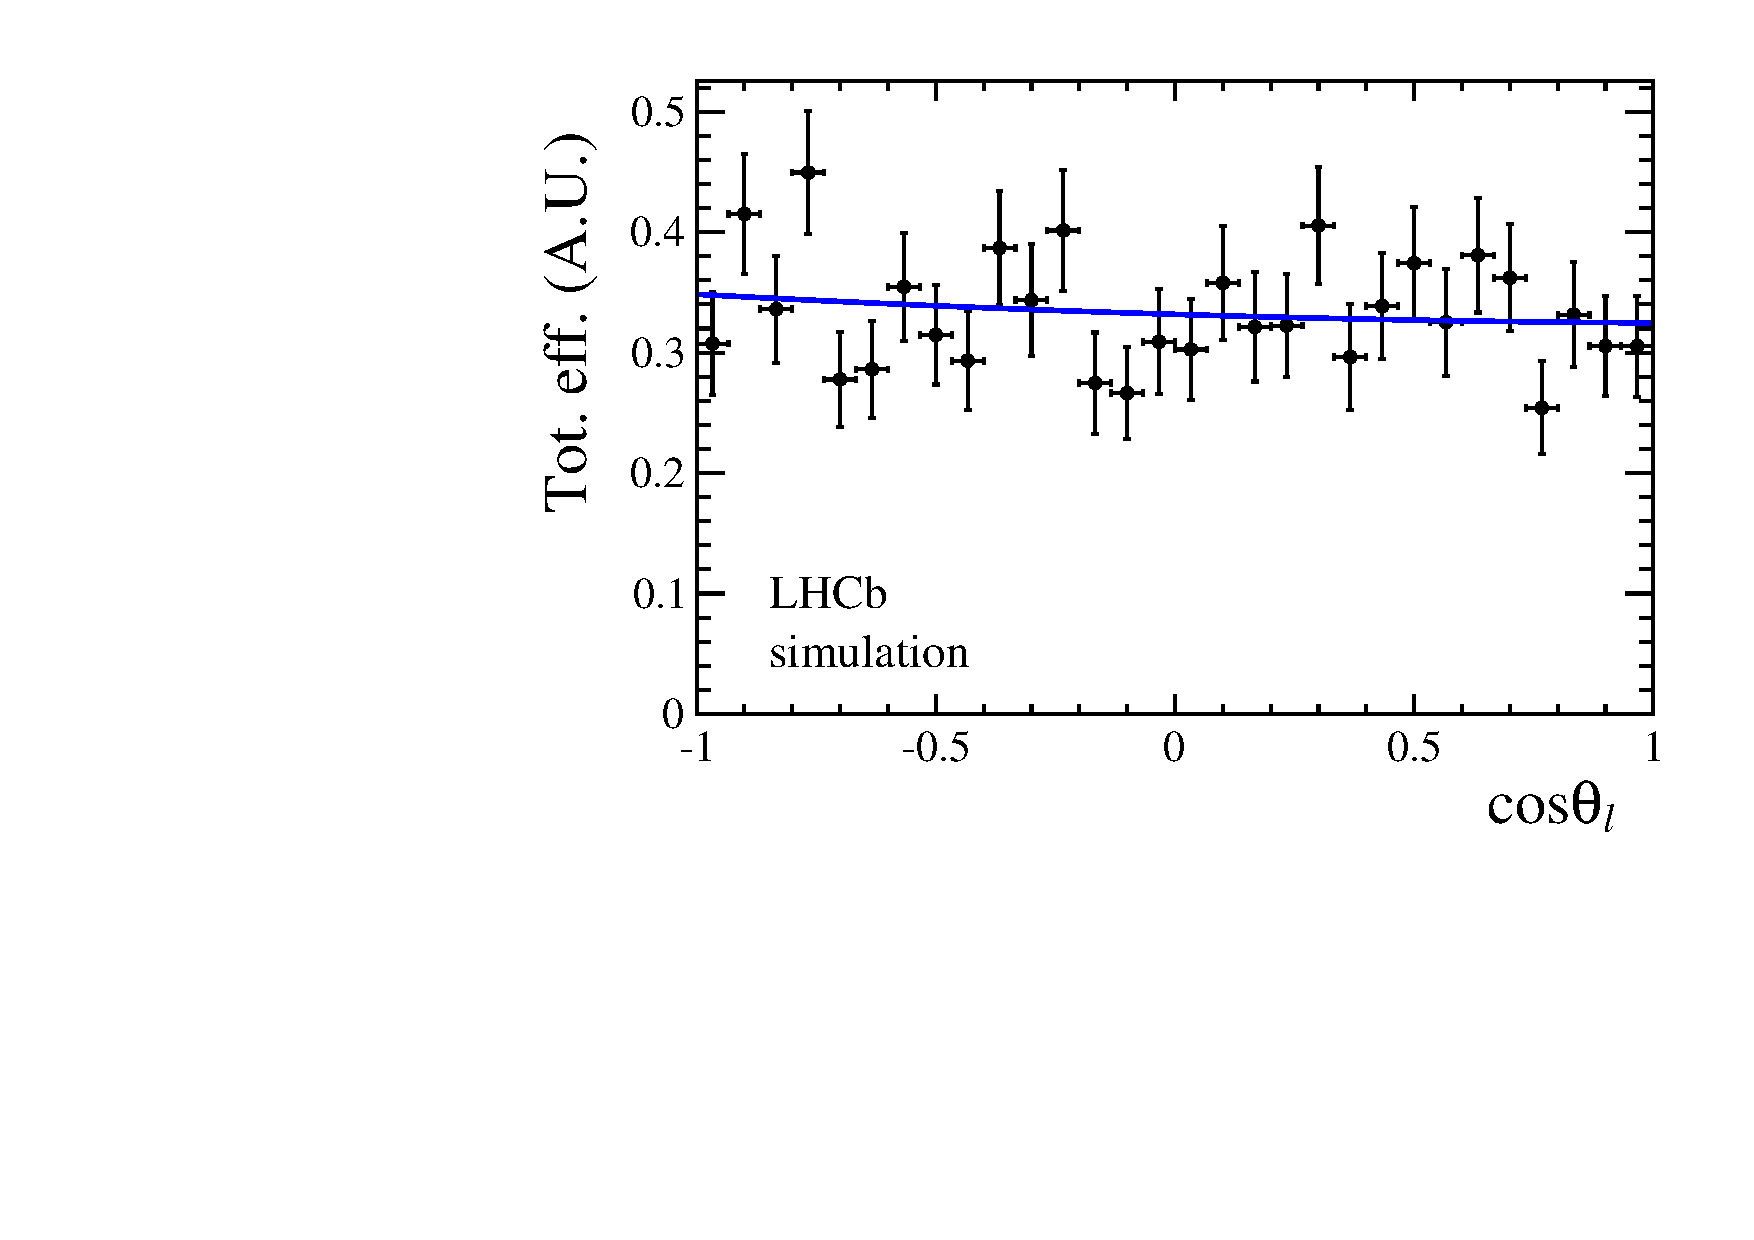
\includegraphics[width=0.45\textwidth]{images_and_tables/Angular/LLeffFit_q2_1500_2000.pdf}
%%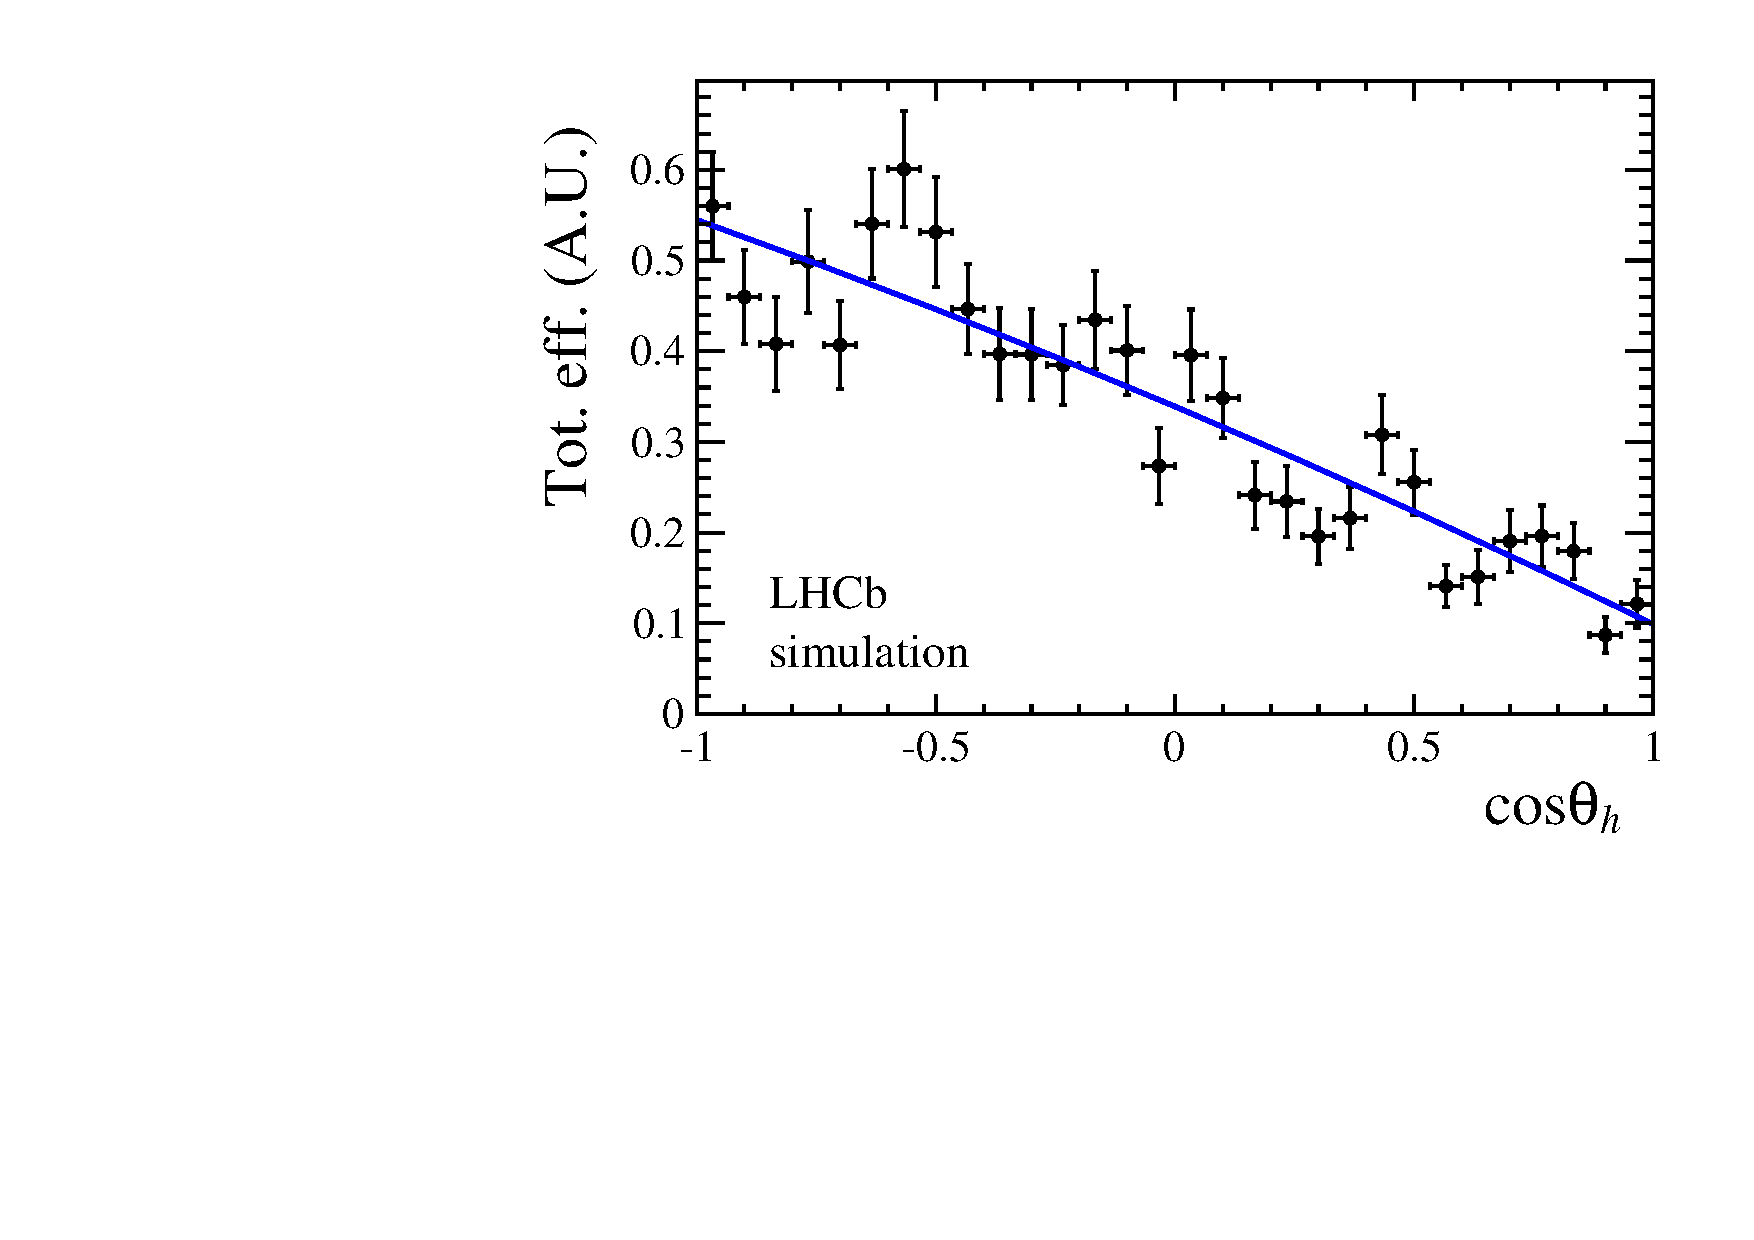
\includegraphics[width=0.45\textwidth]{images_and_tables/Angular/LLeffFitB_q2_1500_2000.pdf}
%%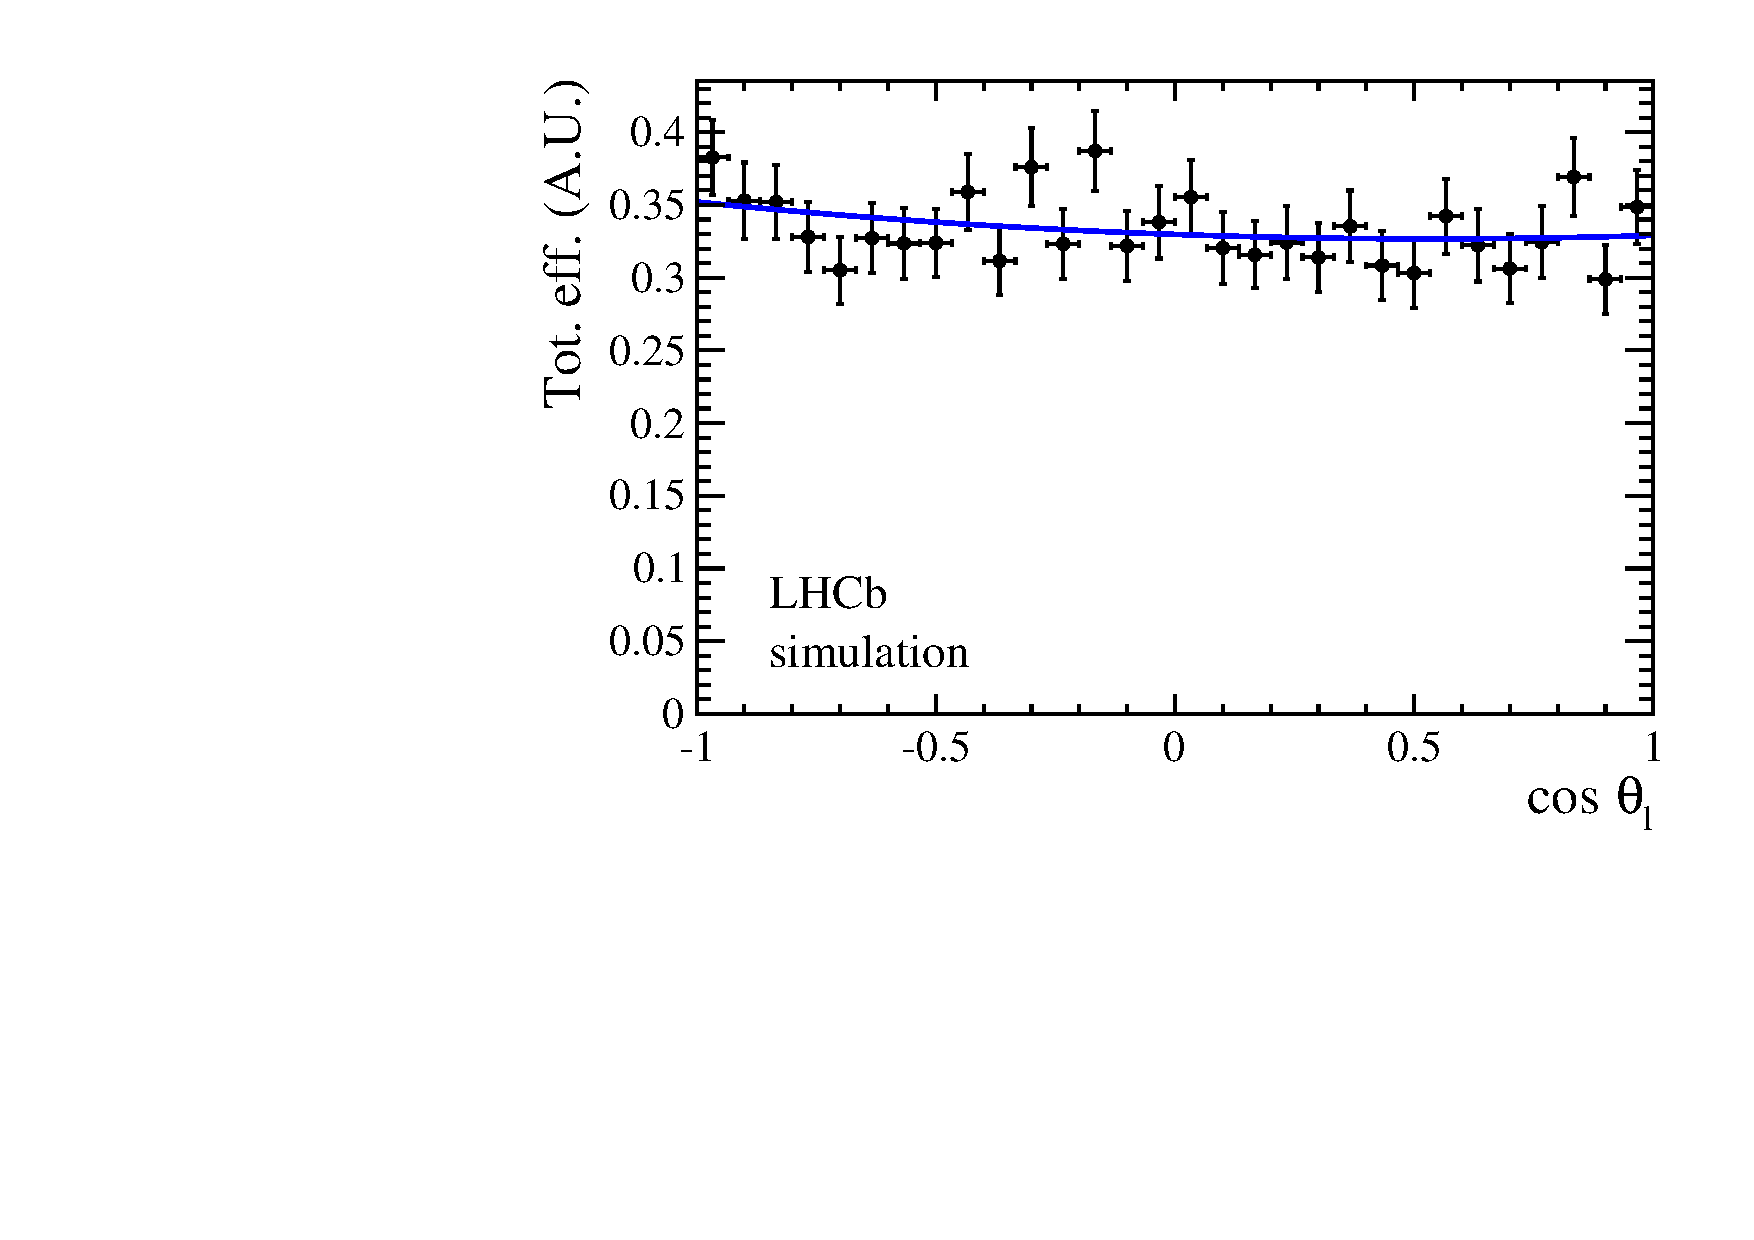
\includegraphics[width=0.45\textwidth]{images_and_tables/Angular/DDeffFit_q2_1500_2000.pdf}
%%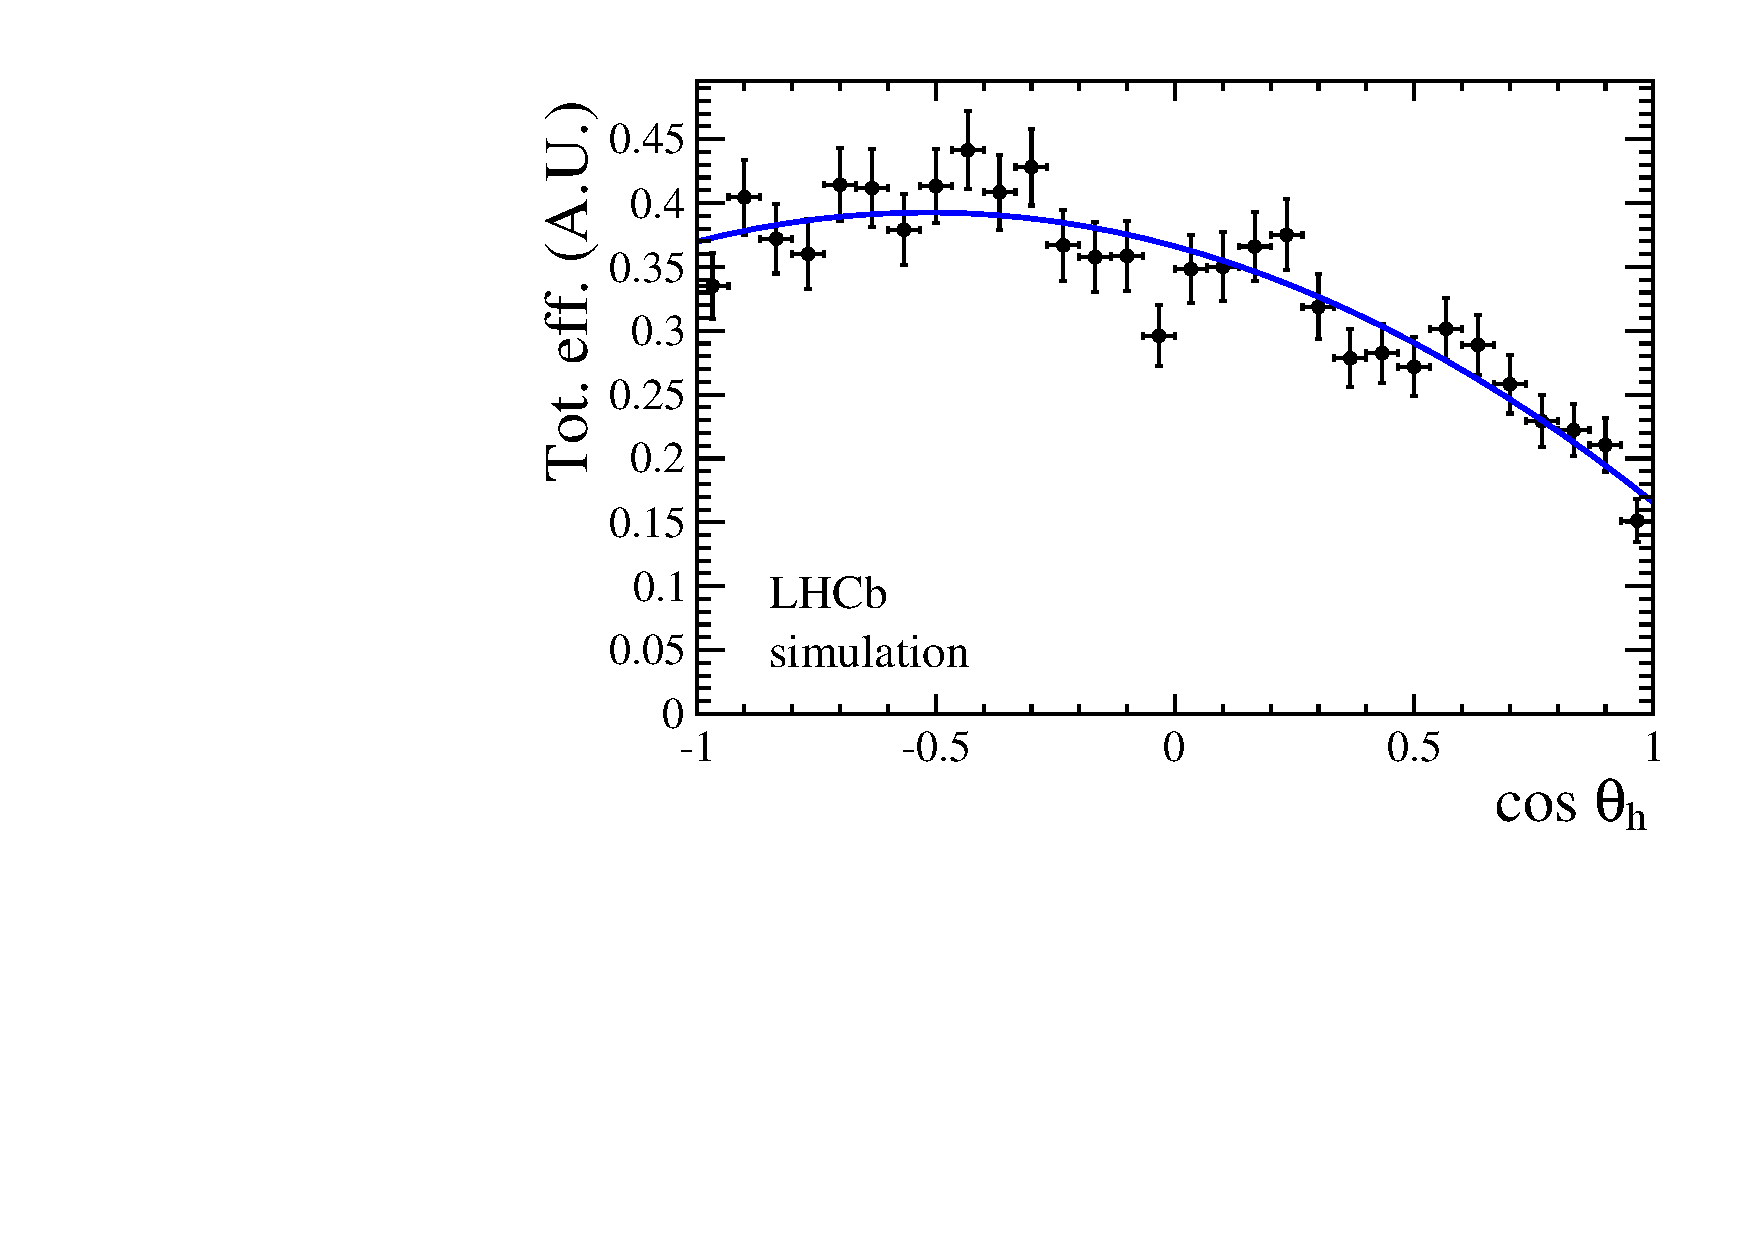
\includegraphics[width=0.45\textwidth]{images_and_tables/Angular/DDeffFitB_q2_1500_2000.pdf}
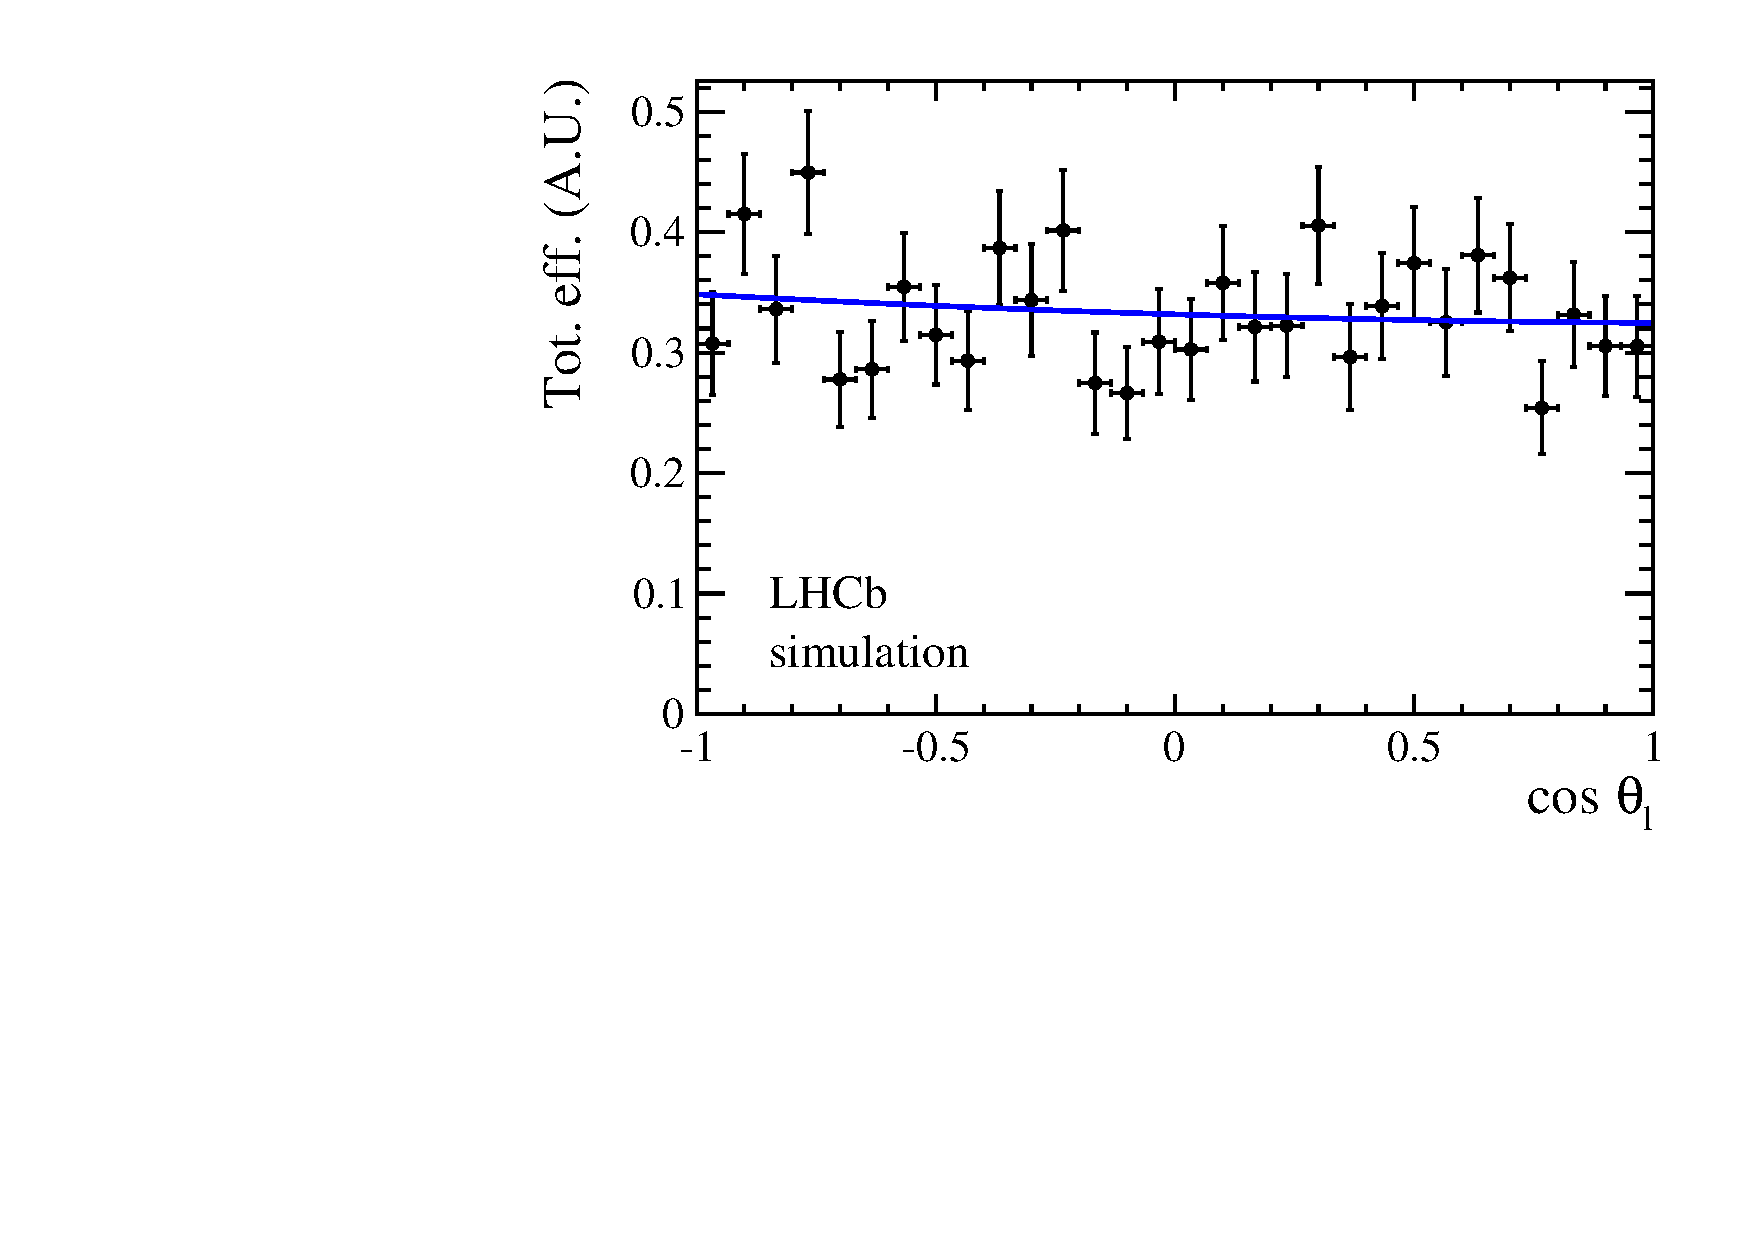
\includegraphics[width=0.45\textwidth]{figure6a.pdf}
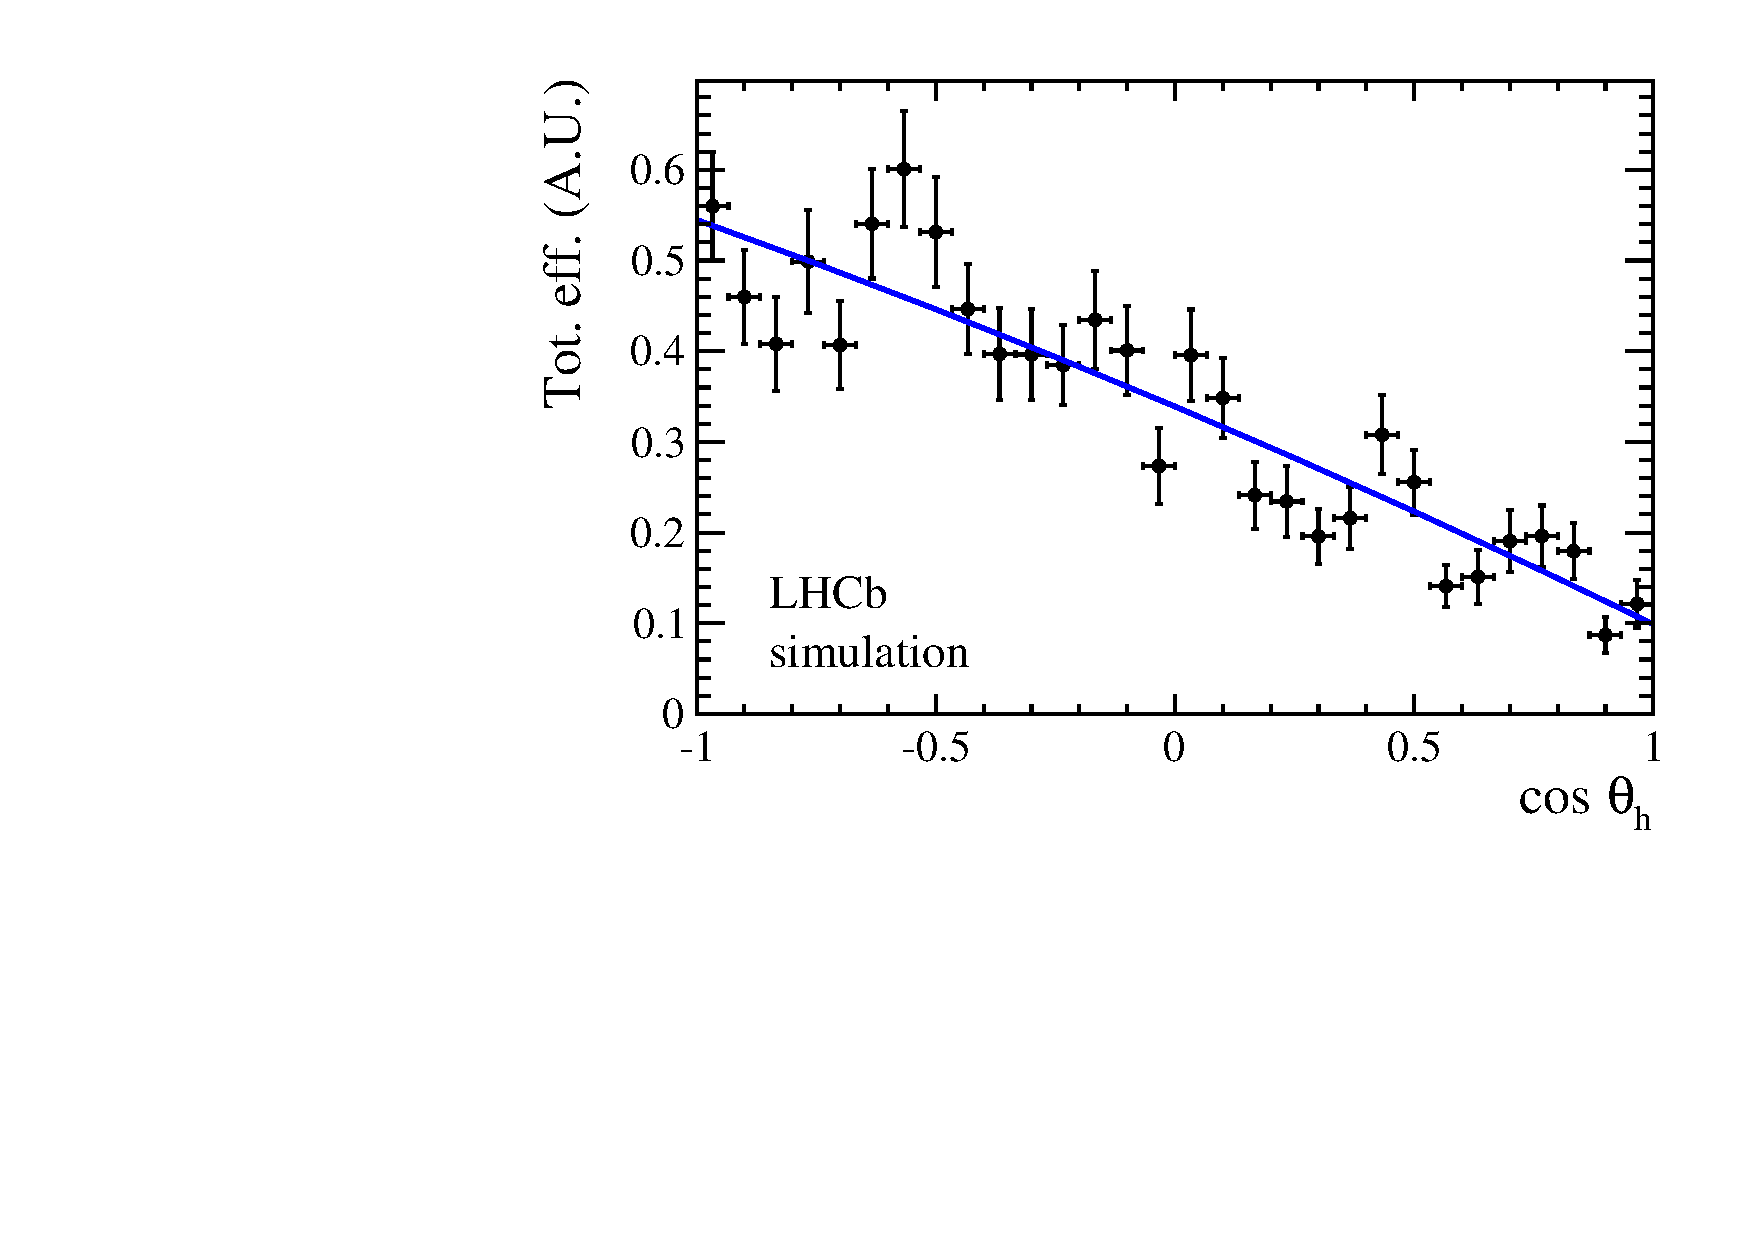
\includegraphics[width=0.45\textwidth]{figure6b.pdf}
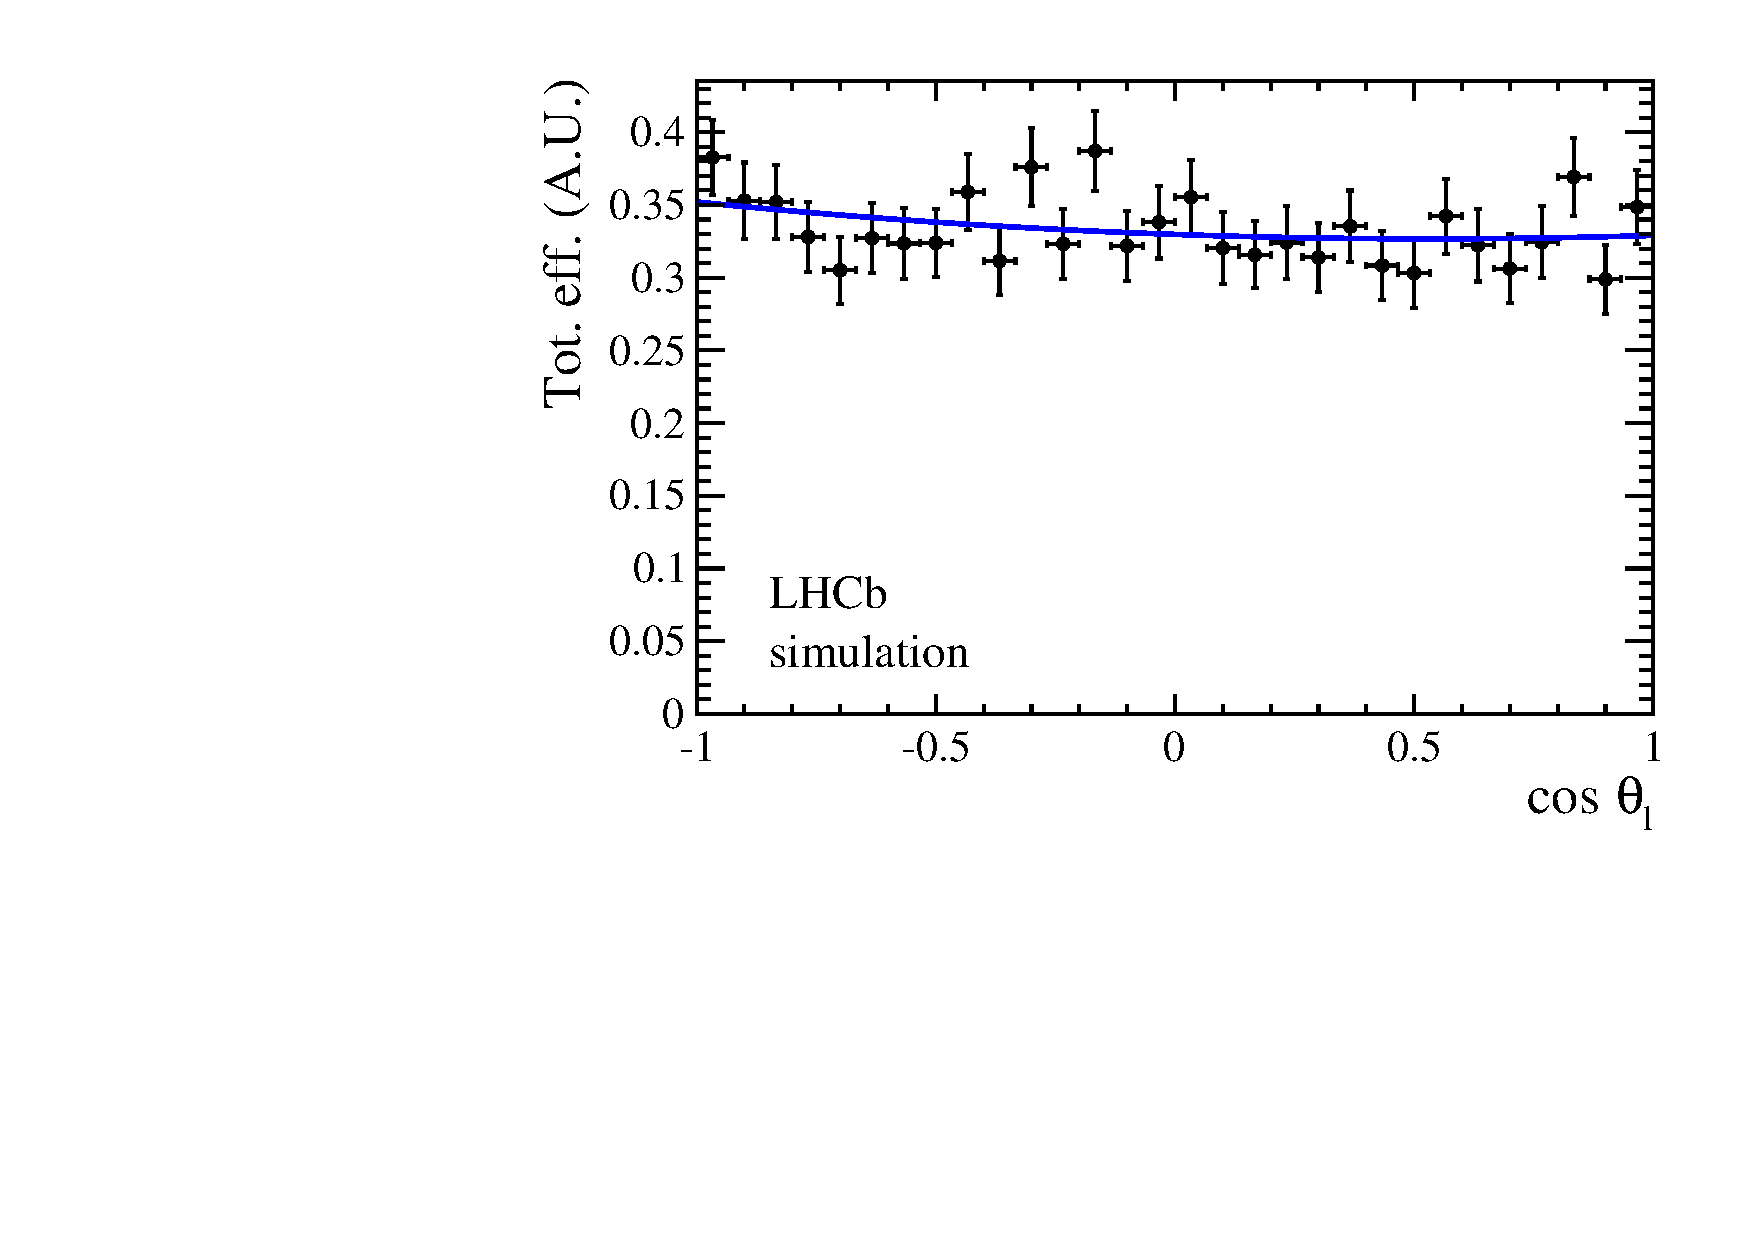
\includegraphics[width=0.45\textwidth]{figure6c.pdf}
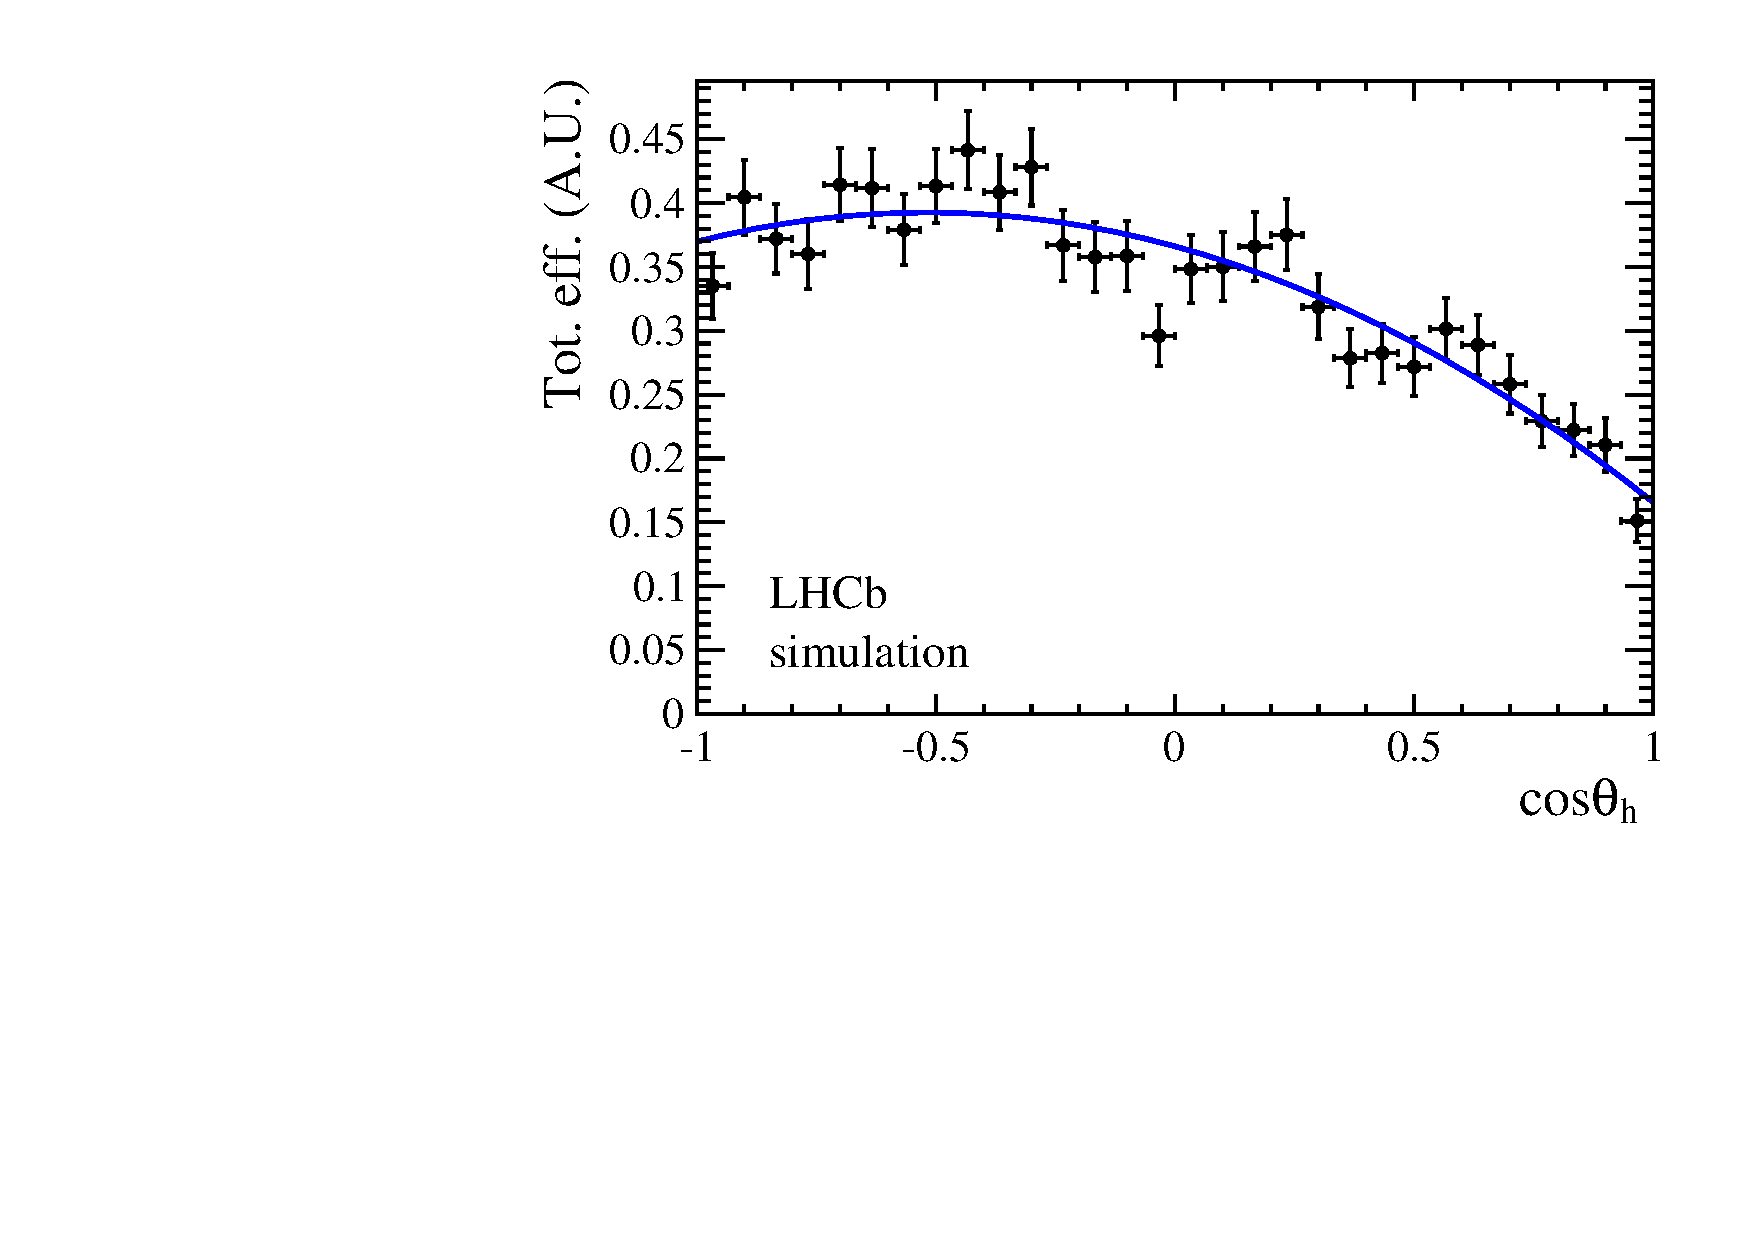
\includegraphics[width=0.45\textwidth]{figure6d.pdf}

\caption{Angular efficiencies as a function of (left)
  $\cos\theta_\ell$ and (right) $\cos\theta_h$ for (upper) long and
  (lower) downstream candidates, in the interval $15 < \qsq < 20$
  \gevgevcccc, obtained using simulated events.  The (blue) line shows
  the fit that is used to model the angular acceptance in the fit to
  data. }
\label{fig:AngEff}
\end{figure}


\begin{figure}[tbp]
\centering
%%ncludegraphics[width=0.49\textwidth]{images_and_tables/Angular/fit_q2_1500_2000_All_cosThetaL.pdf}
%%ncludegraphics[width=0.49\textwidth]{images_and_tables/Angular/fit_q2_1500_2000_All_cosThetaB.pdf}
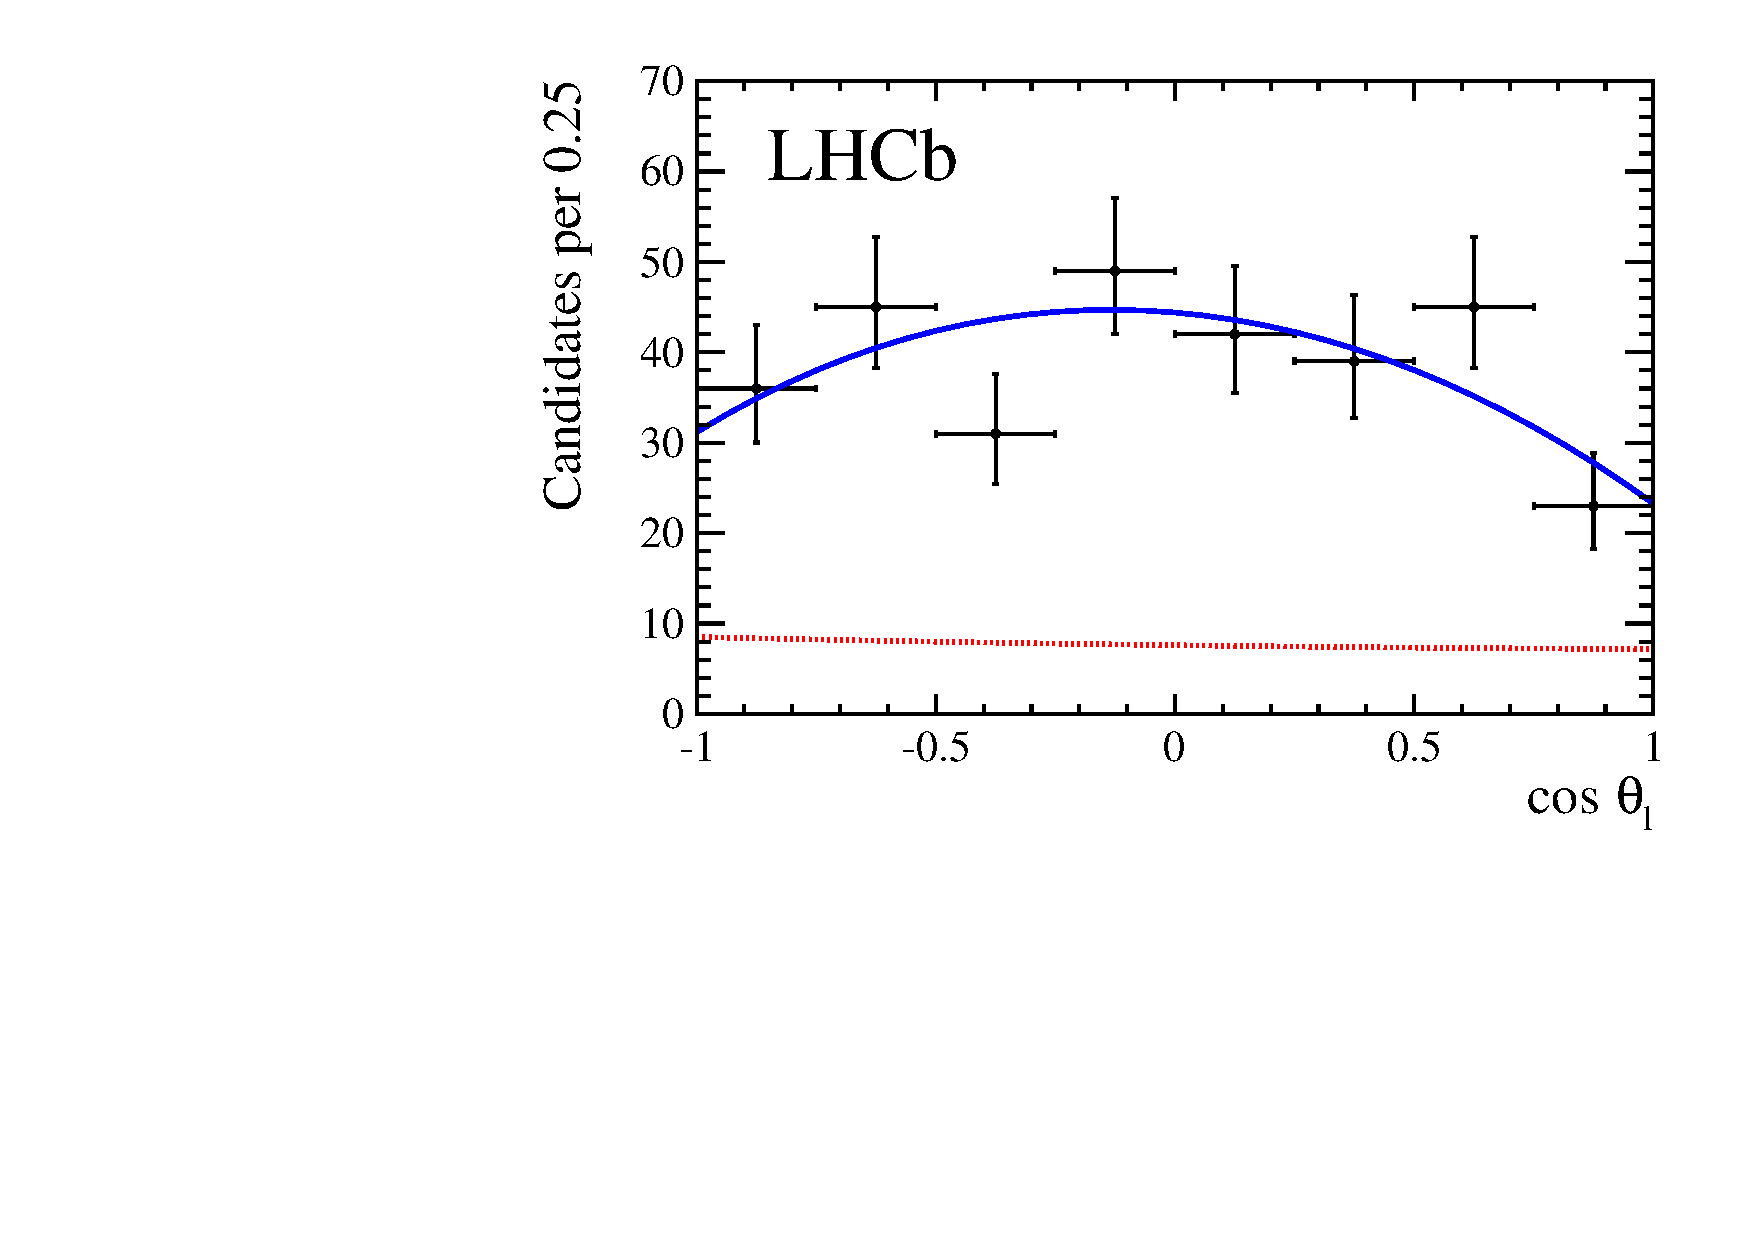
\includegraphics[width=0.49\textwidth]{figure7a.pdf}
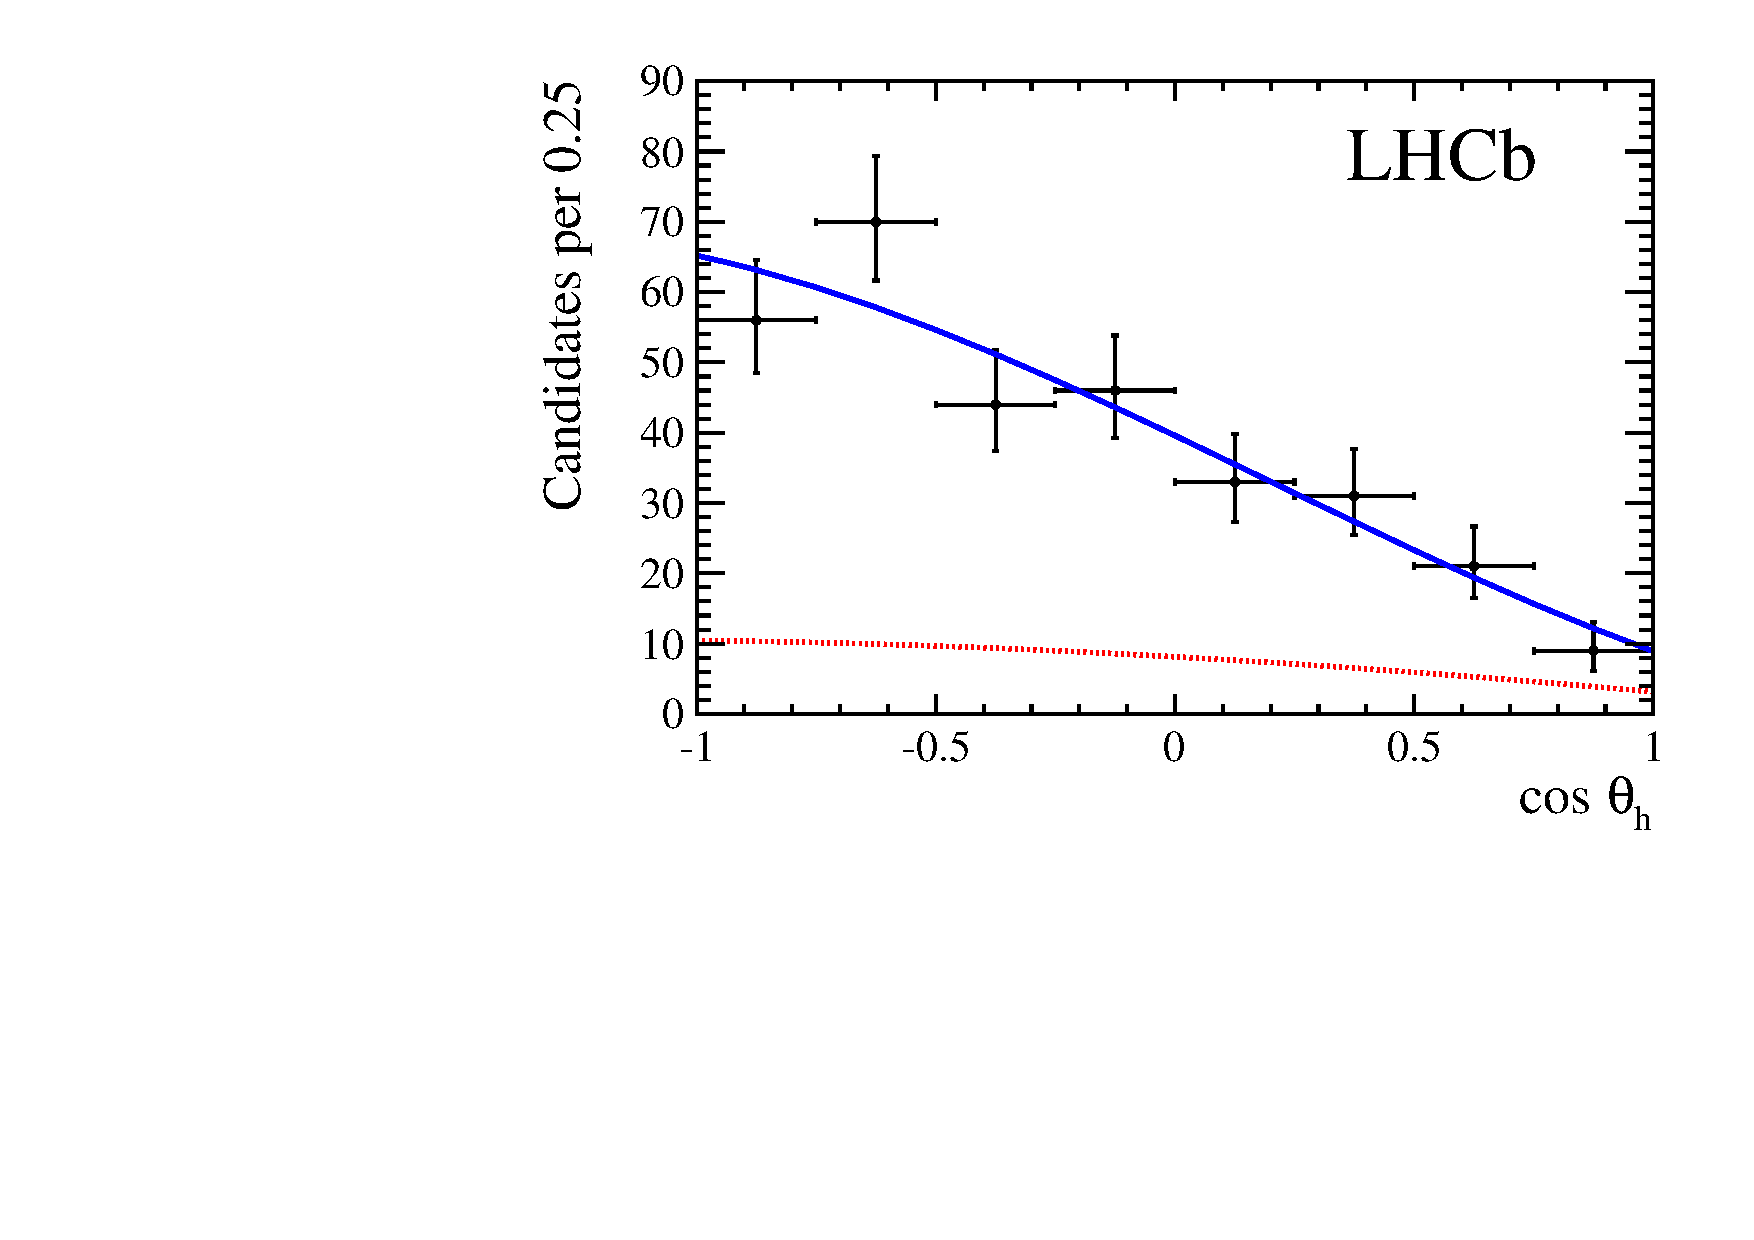
\includegraphics[width=0.49\textwidth]{figure7b.pdf}
\caption{Angular distributions as a function of (left) $\cos
  \theta_\ell$ and (right) $\cos \theta_h$, for candidates in the
  integrated $15 < \qsq <20$ \gevgevcccc interval with the overall fit
  function overlaid (solid blue). The (red) dotted line represents the
  combinatorial background.}
\label{fig:AngDistrib}
\end{figure}

The angular fit is performed simultaneously for the samples of downstream and
long candidates, 
using separate acceptance and background functions for the two
categories while keeping the angular observables as shared parameters.
Angular distributions are shown in Fig.~\ref{fig:AngDistrib} where the
two candidate categories are combined. 
